

\section{Motivación e identificación del problema}

La utilidad de Wikipedia como la mayor fuente información (en forma de artículos sobre eventos, personajes, definiciones, conceptos, locaciones y entre otros...) se debe a su extensa red de colaboradores.

Cada vez que estos ejecutan una acción en la Wikipedia -ya sea si aportan artículo complejo o corrigen una tilde- dejan una huella llamada metadatos. Estos "rastros", conformados por fechas, número de líneas editadas, direcciones IP y demás, son de suma importancia para analistas de datos.

Estos, si tienen la experiencia, la práctica y tienen el tiempo para dedicarse a estudiar la API de Wikipedia; pueden tomar la metadata, procesarla y generar gráficos para buscar patrones de interés. 

El proceso es largo, y su complejidad limita quien puede formar parte. Si se tuviera una solución donde aquellos interesados "no técnicos" puedan ayudar y donde los interesados experimentados no tengan que dedicarle exhaustivas cantidades de tiempo para poder aportar.

Este trabajo final de grado propone entonces una herramienta que facilita esta laboriosa tarea para todo tipo de usuarios. 
Dándoles una interfaz fácil de usar y flexible para generar gráficos 


\section{Objetivos del trabajo}


\subsection{Objetivo General}
% TODO : Hacer Objetivo General
Crear una nueva versión del front-end de wikimetrics y extender con funcionalidades pertinentes para fomentar discusión sobre los artículos

\subsection{Objetivos Específicos}
% TODO: Objectivos Específicos

\begin{itemize}
    \item Implementar una aplicación web responsive que ofrezca las funcionalidades requeridas por un watcher de un wiki y que pueda ser reconocida por los motores de búsqueda.
    \item Consumir y extender la API de wikimetrics para desarrollar una aplicación web que habilite a sus usuarios construir y visualizar gráficas
    \item Definir los requerimientos de la aplicación
    \item Utilizar un método ágil para el desarrollo de la aplicación.
    \item Realizar el despliegue y puesta en producción de la aplicación
\end{itemize}

\section{Estrategia de solución y método de desarrollo ágil a utilizar}

\subsection{Desarrollo Rápido de Aplicaciones (RAD)}

% TODO: revisar e iterar

El desarrollo rápido de aplicaciones es una metodología de desarrollo que prioriza la creación rápida y prototipos y la retroalimentación rápida sobre ciclos prolongados de desarrollo y prueba. Con el uso de RAD, los desarrolladores pueden realizar múltiples iteraciones y actualizaciones al software rápidamente sin la necesidad de iniciar un cronograma de desarrollo desde cero cada vez.

Esta metodología de desarrollo fue creada por James Martin en el año 1980 en IBM y fue formalizada con la publicación del libro \emph{Rapid Application Development} en 1991.

\begin{figure}[H]
    \centering
    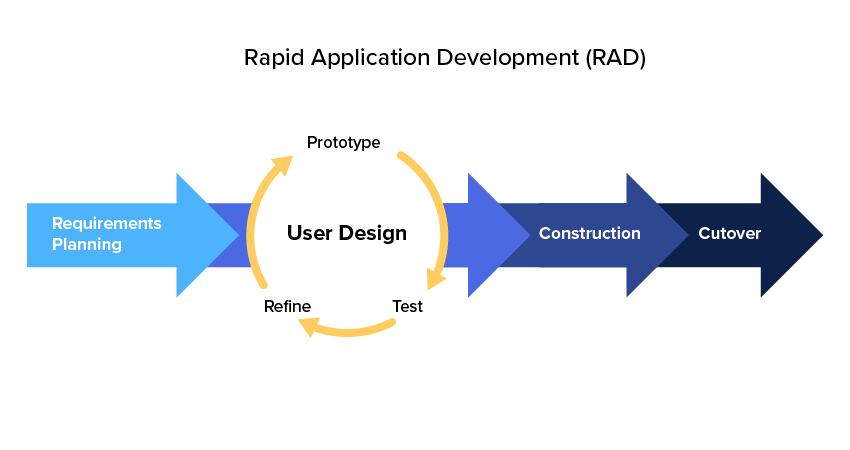
\includegraphics[width=\textwidth]{Rapid-application-development.png}
    \caption{Fases del Desarrollo Rápido de Aplicaciones (enfoque de James Martin)}
    \label{fig:Rapid-application-development}
\end{figure}

\subsubsection{Fases del Desarrollo Rápido de Aplicaciones}

Según el enfoque de James Martin \cite{RADJamesMartin} el Desarrollo Rápido de Aplicaciones se divide en las siguientes fases:

\begin{itemize}
    \item \textbf{Fase de planificación:} Esta fase es equivalente a una reunión de alcance del proyecto. Aunque la fase de planificación se condensa en comparación con otras metodologías de gestión de proyectos.

          Durante esta etapa, los desarrolladores, los clientes (usuarios de software) y los miembros del equipo se comunican para determinar los objetivos y las expectativas del proyecto, así como los problemas actuales y potenciales que deben abordarse durante la construcción.

    \item \textbf{Fase de diseño:} Durante esta fase, los usuarios interactúan con analistas de sistemas y desarrollan modelos y prototipos que representan todos los procesos, entradas y salidas del sistema.

          Todos los errores y problemas se resuelven en un proceso iterativo. El desarrollador diseña un prototipo, el cliente (usuario) lo prueba y luego se reúnen para comunicar qué funcionó y qué no.

    \item \textbf{Fase de construcción:} Esta etapa toma los prototipos y el sistema en su fase beta resultado de la etapa de diseño y lo convierte en un modelo funcional.

          Debido a que la mayoría de los problemas y cambios se abordaron durante la minuciosa fase de diseño iterativo, los desarrolladores pueden construir el modelo de trabajo final más rápidamente que siguiendo un enfoque tradicional de gestión de proyectos.

    \item \textbf{Fase de transición:} Esta es la fase de implementación donde el producto terminado va al lanzamiento. Incluye conversión de datos, pruebas y cambio al nuevo sistema, así como capacitación de usuarios.

          Todos los cambios finales se realizan mientras los programadores y los clientes continúan buscando errores en el sistema.

\end{itemize}


\section{Trabajos similares, diferencias y ventajas de la solución a desarrollar}

Siendo Wikimedia y Wikipedia las más grandes comunidades y organizaciones dedicadas a recopilar datos, es lógico pensar que tiene consigo una abundante cantidad de seguidores capacitados y apasionados por aportar lo que puedan. A continuación se detallará el estado actual de las herramientas existentes para explorar la Wikipedia.

Estas herramientas cumplen diferentes objetivos:

\begin{enumerate}
    \item Identificar posibles candidatos para ser administrador.
    \item Identificar peleas de edición.
    \item Proveer una forma visual de ver el desarrollo general de los artículos (crecimiento de artículo, detection de actividad maliciosa, entre otras cosas).
    \item Hacer uso de la información para proveer interfaces educativas tales como cronologías.
\end{enumerate}


\subsection{Toolforge}

Es una suite de herramientas estadísticas para las páginas, usuarios, wikis de Wikimedia. Entre las herramientas hosteadas más populares de toolforge se encuentra 

\begin{itemize}
    \item URL del proyecto \url{https://wikitech.wikimedia.org/wiki/Portal:Toolforge}
\end{itemize}

Comenzando con el proyecto madre de Wikimedia, este gigante sirve de plataforma para que colaboradores técnicos puedan usar servidores de Wikipedia para desarrollo y para poder levantar aplicaciones que mejoren la experiencia de todos los colaboradores de Wikipedia.
\\
Este proyecto es particularmente interesante porque podría ser un medio por el cual la aplicación WikiMetaView y sus dependencias podrían ser servidas al público.

\url{https://www.wikidata.org/wiki/Wikidata:Tools/Visualize_data}

\subsection{Sigma - Summary}

Esta herramienta creada por el usuario Sigma\(\Sigma\) permite obtener el historial de contribuciones de un usuario y filtrar las ediciones por una palabra clave. Tal como se puede observar en la imagen \ref{fig:sigma_summary}, el resultado de buscar el usuario \say{Clarityfiend} y filtrar por la palabra \say{space} es similar al que se puede encontrar en la lista de contribuciones por usuario de Wikipedia \cite{UserClarityfiend}, con el beneficio de poder filtrar por palabras claves.

\begin{itemize}
    \item URL del proyecto \url{https://sigma.toolforge.org/summary.py}
\end{itemize}

\begin{figure}[H]
    \centering
    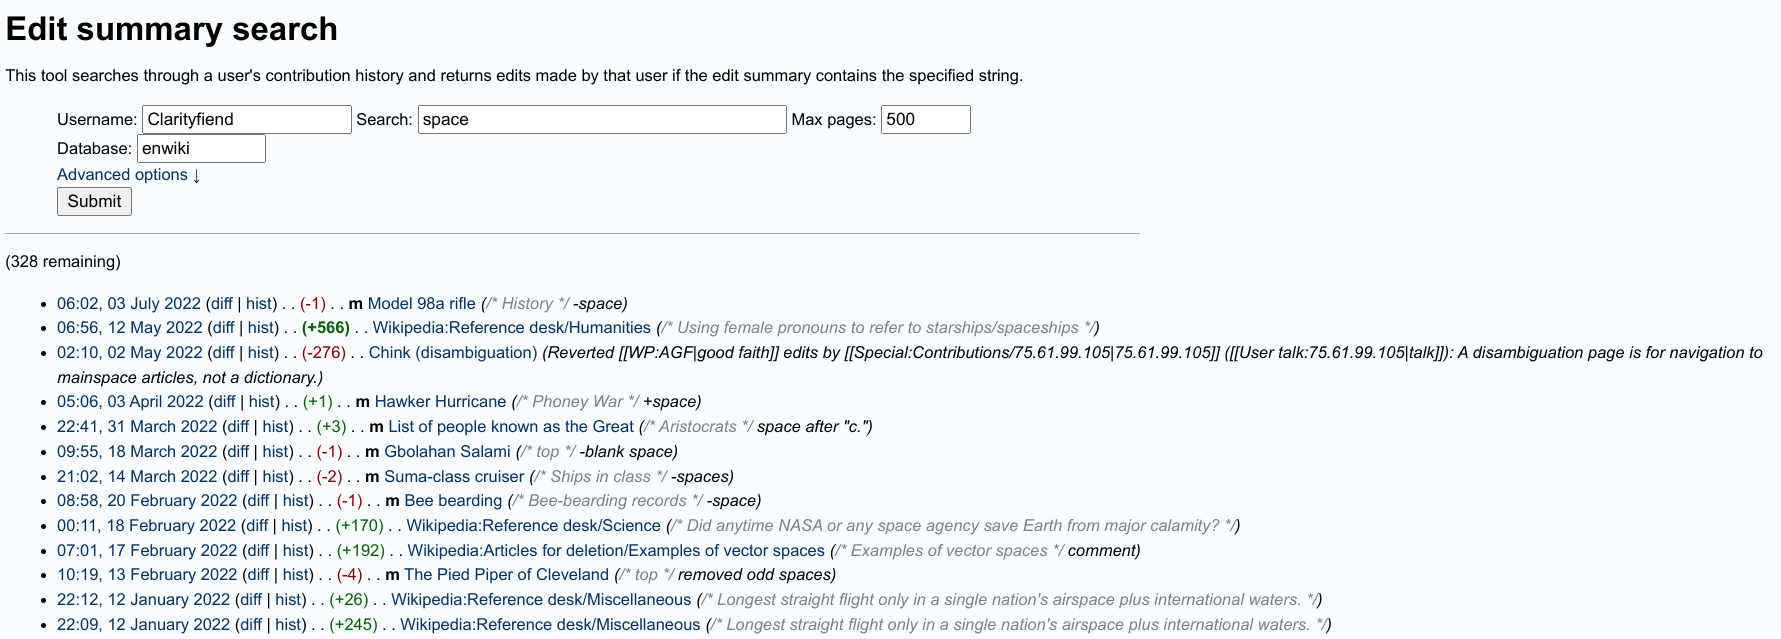
\includegraphics[width=\textwidth]{proyectos-relacionados/sigma-summary.png}
    \caption{Sigma Summary}
    \label{fig:sigma_summary}
\end{figure}

\subsection{Histropedia Timeline}

\begin{itemize}
    \item URL del proyecto \url{http://histropedia.com/timeline/}
\end{itemize}

Es una herramienta que permite visualizar diferentes eventos en forma de línea de tiempo interactiva, usando el servicio de Wikidata para consultas Sparql \cite{WikidataSparql}. Es usada como herramienta educativa por distintas entidades como el Museo del Prado para que los usuarios puedan visualizar de forma sencilla el arte que se expone, tal como se puede observar en la imagen \ref{fig:museo-de-prado-timeline}. Además, la línea de tiempo permite asociar cada elemento de la colección con un evento histórico importante, de tal forma que se facilite el aprendizaje y se haga más dinámico.

\begin{figure}[H]
    \centering
    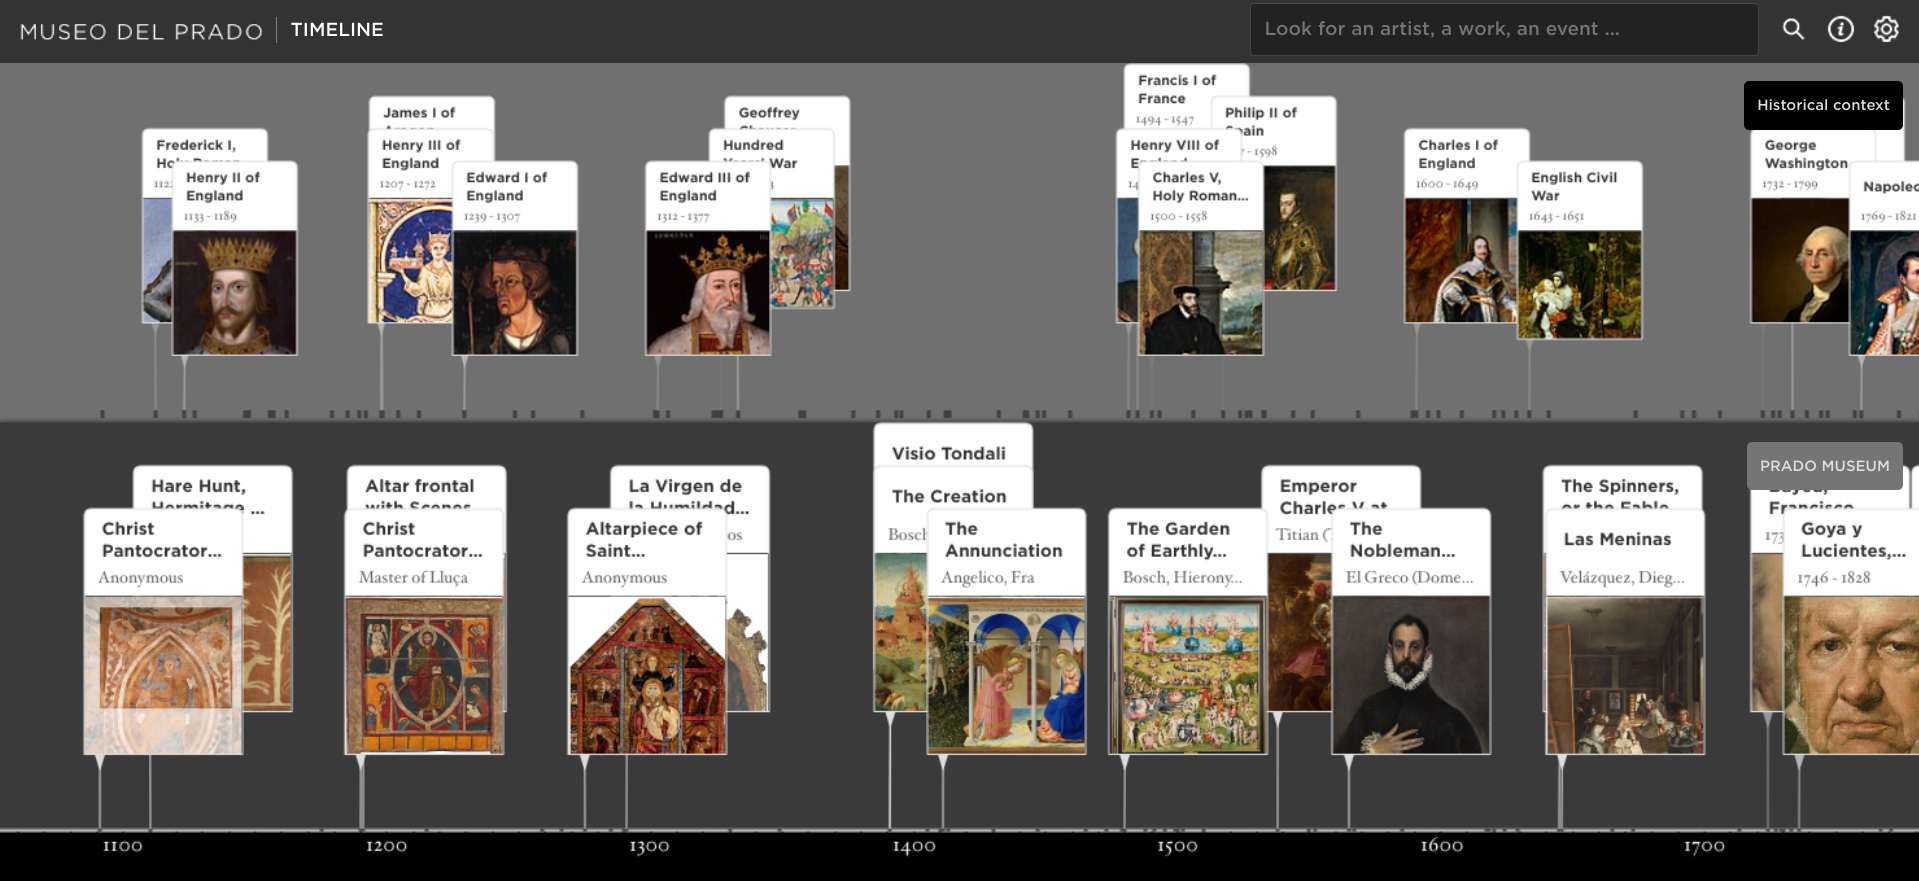
\includegraphics[width=1.0\textwidth]{proyectos-relacionados/museo-del-prado-timeline.png}
    \caption{Línea de tiempo que muestra la colección de arte del Museo del Prado}
    \label{fig:museo-de-prado-timeline}
\end{figure}



\begin{figure}[H]
    \centering
    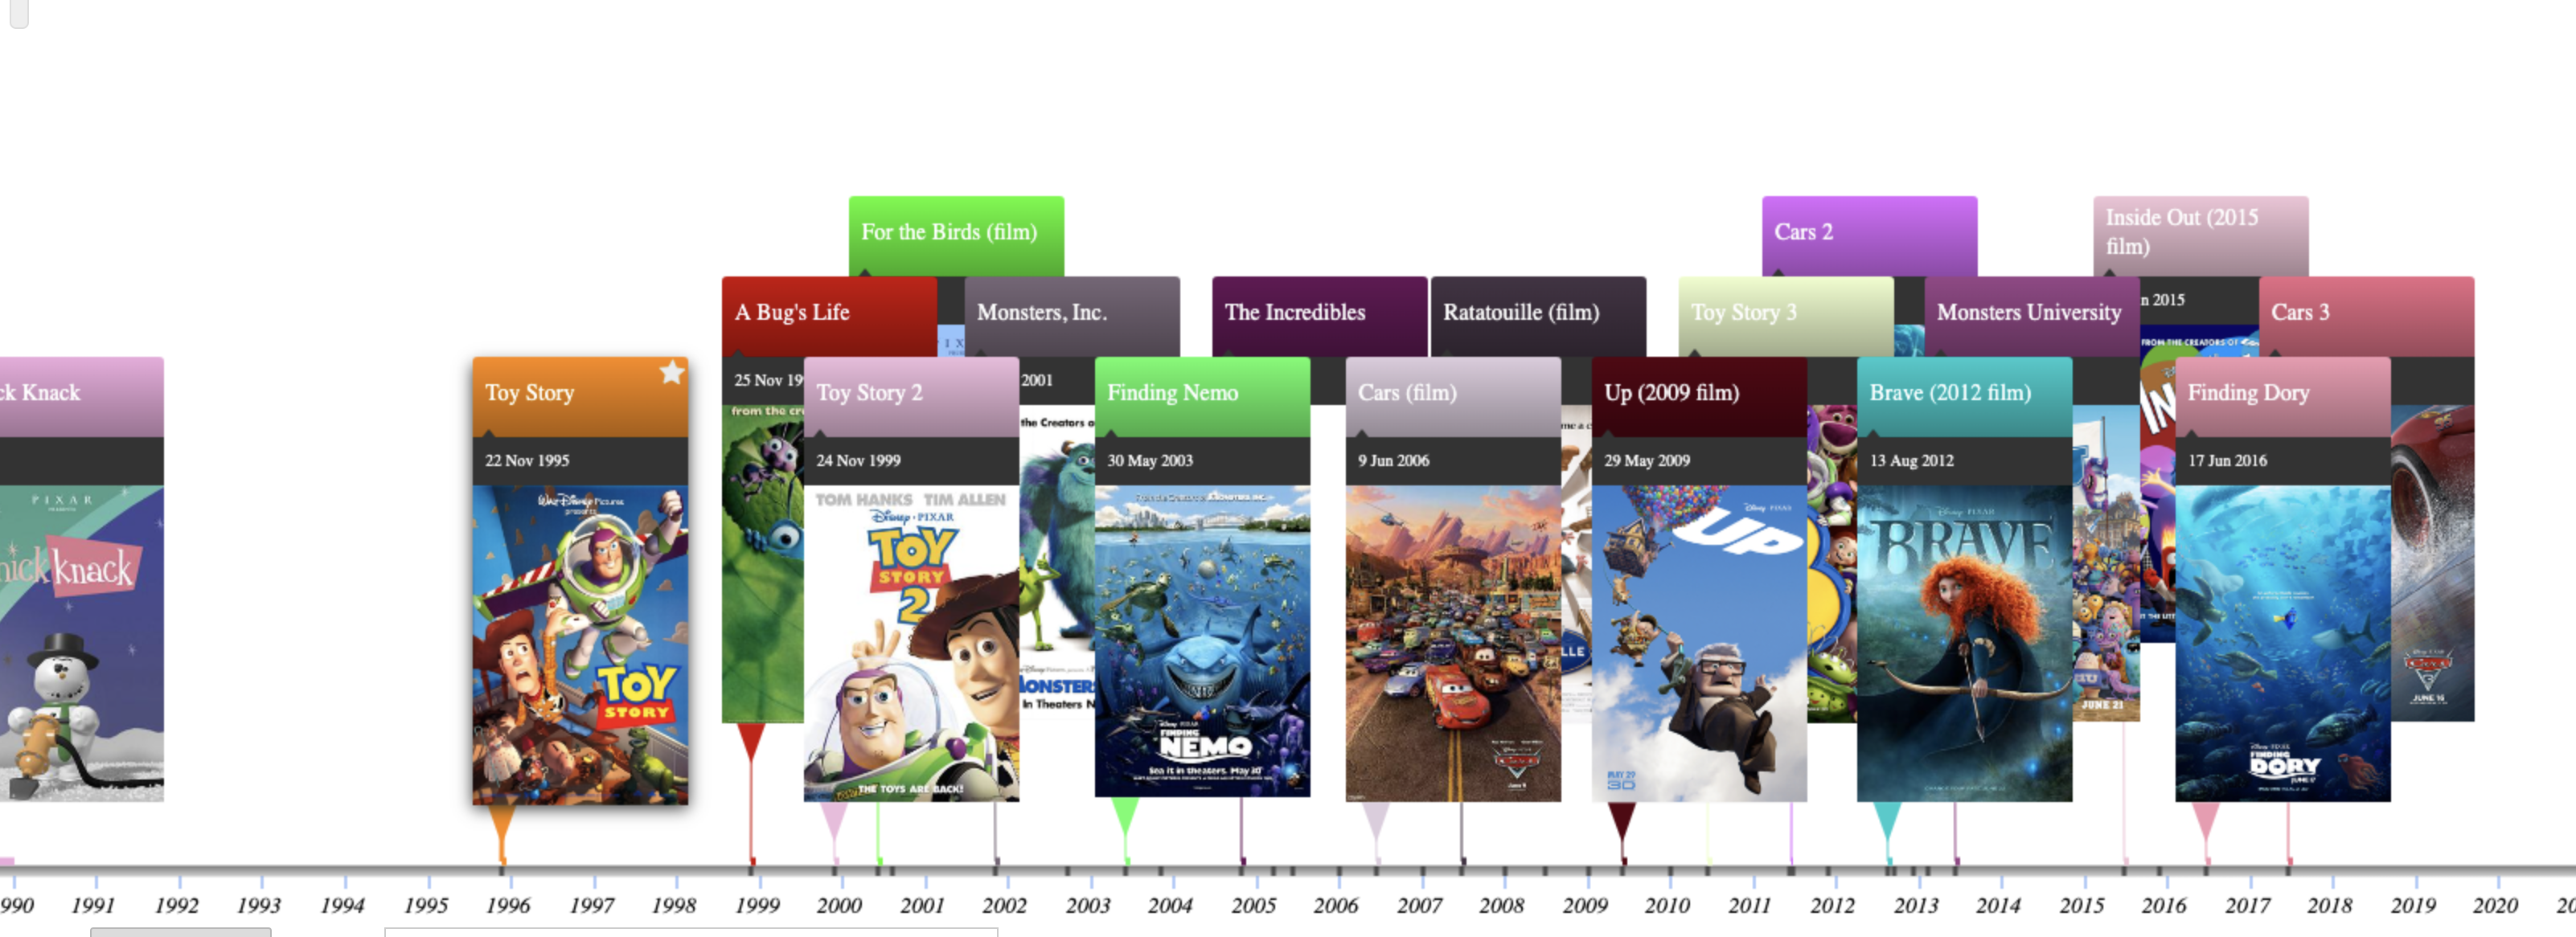
\includegraphics[width=1.0\textwidth]{proyectos-relacionados/histropedia_timeline.png}
    \caption{Histropedia Timeline}
    \label{fig:histropedia_timeline}
\end{figure}


\url{https://en.wikipedia.org/wiki/Wikipedia:Tools}

\url{apersonbot.toolforge.org}
Este set de herramientas está enfocado en supervisar usuarios y sus contribuciones a la Wikipedia

- Candidate Search
- Aadminscore
- Articles for Creation Review History

\subsection{Xtools}
\begin{itemize}
    \item URL del proyecto \url{https://xtools.wmflabs.org/}
\end{itemize}

\subsection{Wiki Replay}
\begin{itemize}
    \item URL del proyecto \url{https://cosmiclattes.github.io/wikireplay/player}
\end{itemize}

Se encarga de mostrar una línea de tiempo con los cambios en un artículo. Esta línea de tiempo
tiene el comportamiento de un reproductor de video y permite que el usuario presione un botón de
reproducir y así ser guiado por como el contenido de un artículo ha ido evolucionando en el tiempo.

\begin{figure}[H]
    \centering
    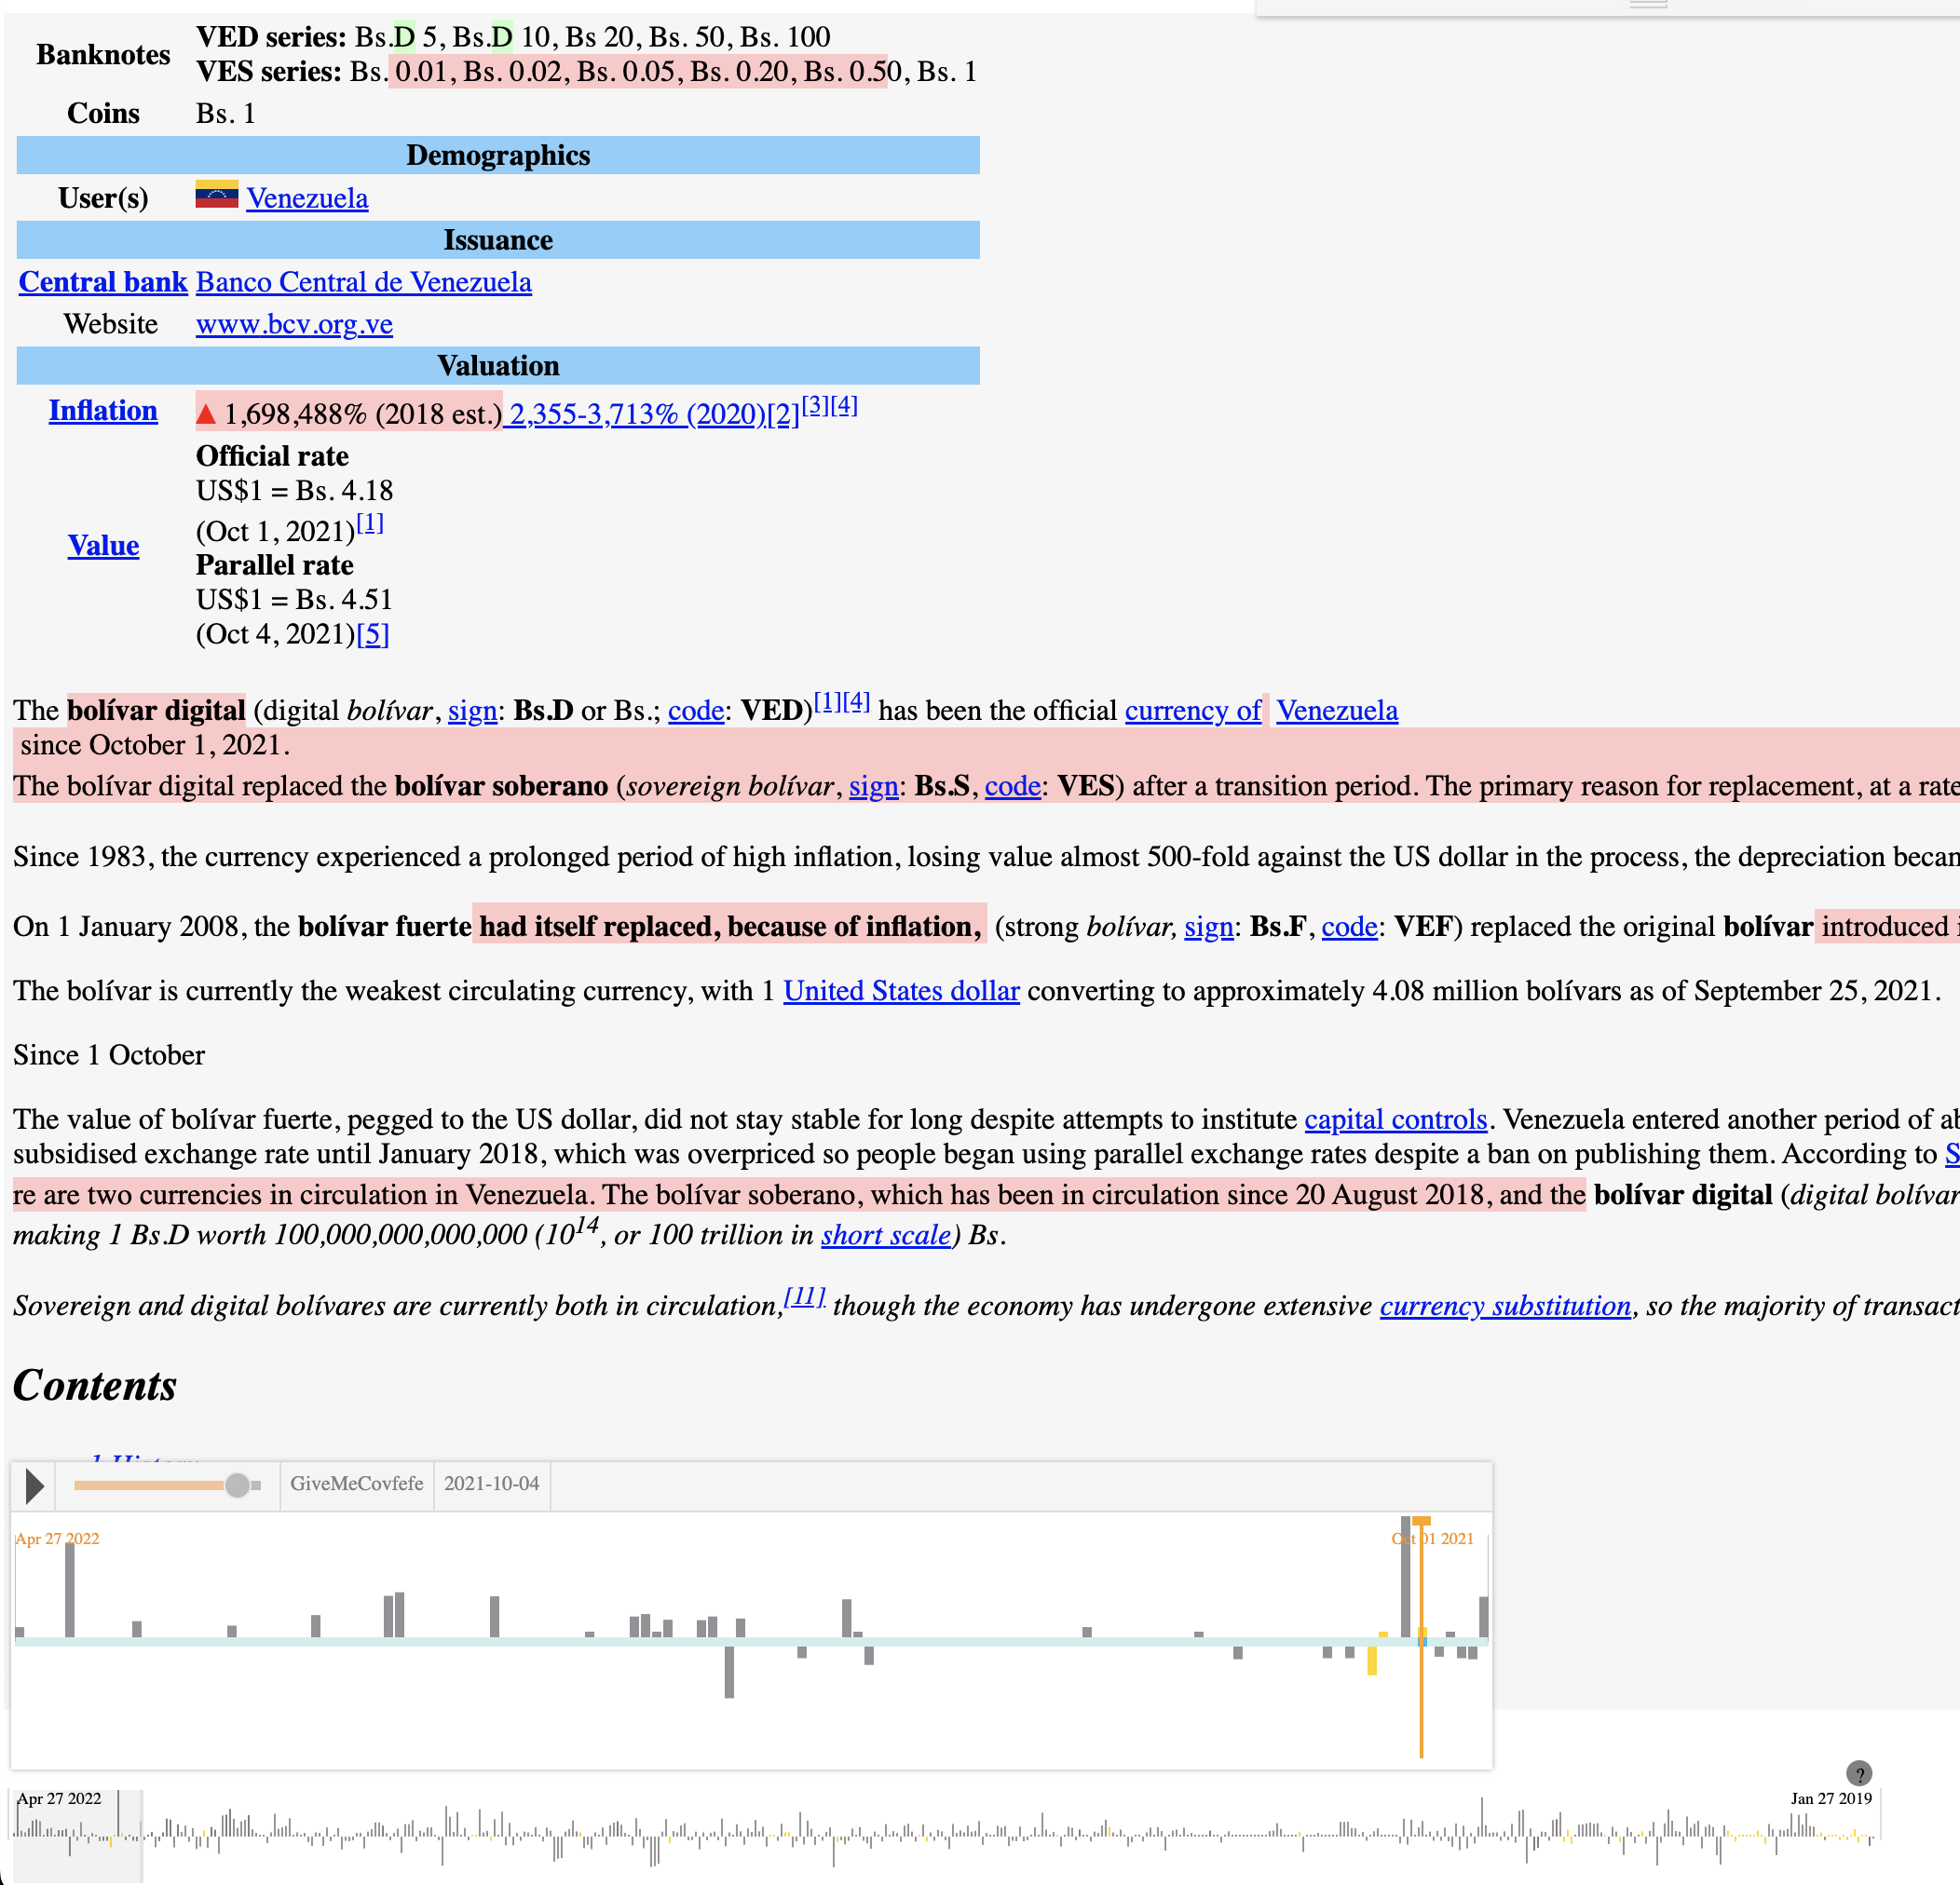
\includegraphics[width=1.0\textwidth]{proyectos-relacionados/wikireplay.png}
    \caption{Interfaz de wikireplay}
    \label{wikireplay}
\end{figure}


\url{https://de.wikipedia.org/wiki/Benutzer:Atlasowa/edit_history_visualization}

\subsection{IBM History Flow tool}

\begin{itemize}
    \item URL del proyecto \url{http://alumni.media.mit.edu/~fviegas/papers/history_flow.pdf}
\end{itemize}

Es una herramienta de análisis de datos exploratorio, la cual utiliza el registro de ediciones que posee Wikipedia para mostrar relaciones entre distintas versiones de un documento. El propósito de esta herramienta es mostrar tendencias o patrones generales del documento, pero al mismo tiempo preservar los detalles para una examinación cercana.

Como se puede observar en la imagen \ref*{fig:history-flow-mechanism} cada barra vertical representa una versión del documento, siendo el largo proporcional a la cantidad de palabras que posee el documento. El color de la versión en toda su extensión permite asociar cada palabra con un usuario, identificando el autor de dicha versión. Por último, se utiliza la distancia entre versiones para separarlas de acuerdo a su fecha y así obtener información extra sobre la frecuencia de edición de cada palabra. Al realizar el procedimiento en la página \say{Brazil} \ref*{fig:brazil-history-flow} se puede observar un evidente incremento en la longitud de las barras verticales, lo que implica un crecimiento drástico del contenido de la página.

\begin{figure}[H]
    \centering
    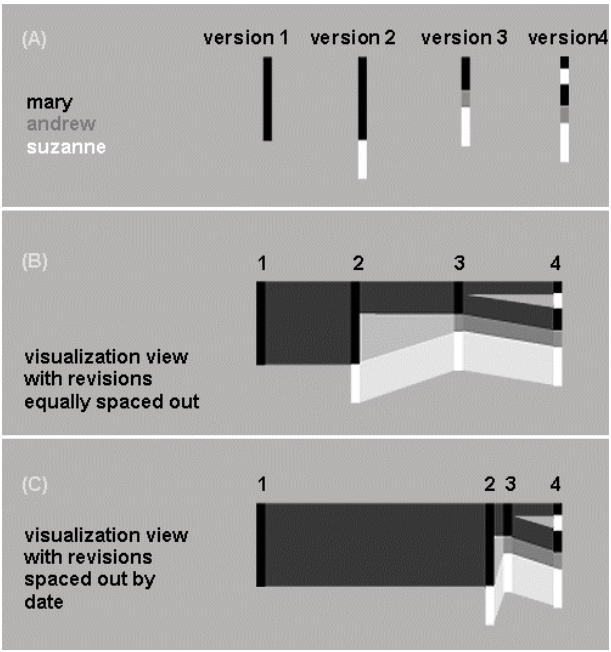
\includegraphics[width=\textwidth]{proyectos-relacionados/history-flow-mechanism.png}
    \caption{Explicación del mecanismo de visualización de History Flow}
    \label{fig:history-flow-mechanism}
\end{figure}

\begin{figure}[H]
    \centering
    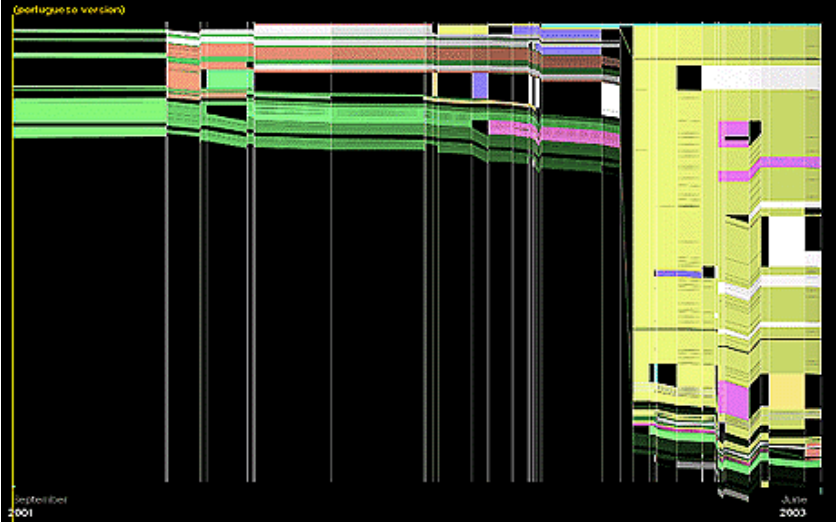
\includegraphics[width=\textwidth]{proyectos-relacionados/brazil-history-flow.png}
    \caption{La página "Brazil" mostrando un crecimiento abrupto y pocas contribuciones anónimas}
    \label{fig:brazil-history-flow}
\end{figure}

\subsection{Wiki History Flow}

\begin{itemize}
    \item URL del proyecto \url{https://github.com/rdmpage/wikihistoryflow}
    \item
\end{itemize}

Es un repositorio que posee varios archivos de PHP que permiten crear el history flow de una página en formato SVG. Este proyecto obtiene las revisiones directamente de Wikipedia haciendo uso de web scrapping y calculando la diferencia entre textos con el paquete de Pear Text\_Diff \cite{pear_text_diff}, para después graficar las diferencias en forma de history flow.

\begin{figure}[H]
    \centering
    \includegraphics[width=\textwidth]{proyectos-relacionados/rdm-historyflow.png}
    \caption{History Flow creado por el proyecto}
    \label{fig:rdm-historyflow}
\end{figure}


\section{Herramientas}
En esta sección se enumerará 

\subsection{Tecnologías para el ambiente de desarrollo}
\begin{itemize}
    \item Visual Studio Code.
    \item Git, como control de versiones.
    \item Navegadores web (Google Chrome, Firefox, etc).
    \item Base de Datos (MongoDB).
    \item Servidor (Nodejs).
    \item Manejador de paquetes de NPM (pnpm).
\end{itemize}

\subsection{Tecnologías o librerías web a utilizar}
\begin{itemize}
    \item Material UI.
    \item Next.js + ReactJS.
    \item Node.
    \item MongoDB.
    \item Fastify.
\end{itemize}

\section{Requerimientos}
\begin{enumerate}
    \item{Una herramienta capaz de visualizar gráficas sobre propiedades de edición de un wiki.}
    \item{Los wikis a visualizar son extraídas del watchlist del usuario autenticado a través de Wikipedia (usando API de MediaWiki).}
    \item{Permitir editar las visualizaciones (alternar tipo de gráfica, cambiar los tipos de datos a visualizar).}
    \item{Los datos a representar en las visualizaciones son proporcionados a través del API Wikimetrics 2.0.}
    \item{La herramienta tiene que ser una aplicación web.}
    \item{La aplicacion tiene que contar con una vista principal que incluya gráfica e información general de cada uno de los wikis del watchlist.}
    \item{Permitir al usuario crear una visualización nueva y guardarla de forma permanente, para este caso es necesario el uso de una base de datos (preferiblemente MongoDB)}
    \item{La aplicación tiene que estar alojada en un servidor, para poder ser accedida de manera remota.}
\end{enumerate}

\section{Prototipo de interfaz}

\subsection{Perfil de Watcher \textbackslash watcher\textbackslash:watcherId}
Para cualquier usuario muestra el perfil de un watcher, en él puedes ver todas las contribuciones de este junto con la lista de visualizaciones que ha creado.
Se permitirá un mínimo de personalización. Y se podrá enlazar el perfil de Wikipedia

\begin{figure}[H]
    \centering
    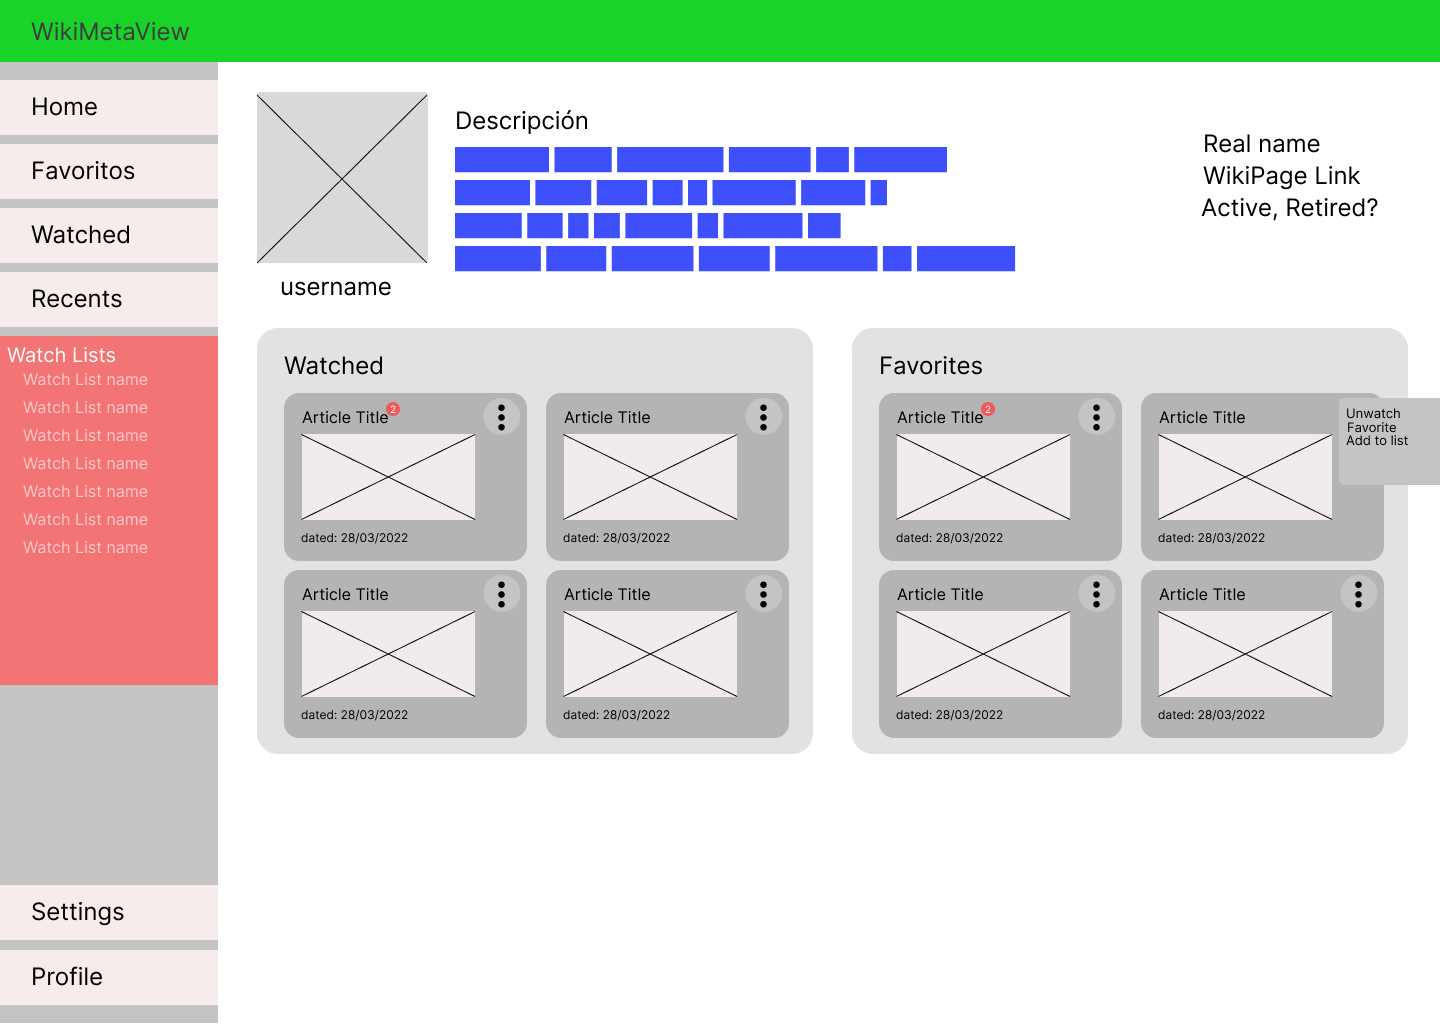
\includegraphics[width=1.0\textwidth]{prototipos/Watcher Profile.png}
    \caption{Prototipo de página de perfil de watcher}
    \label{PrototipoWatchersProfile}
\end{figure}

\subsection{Página principal \textbackslash home}
Para usuarios autenticados, les permite ver diferentes secciones relevantes para ellos

\begin{figure}[H]
    \centering
    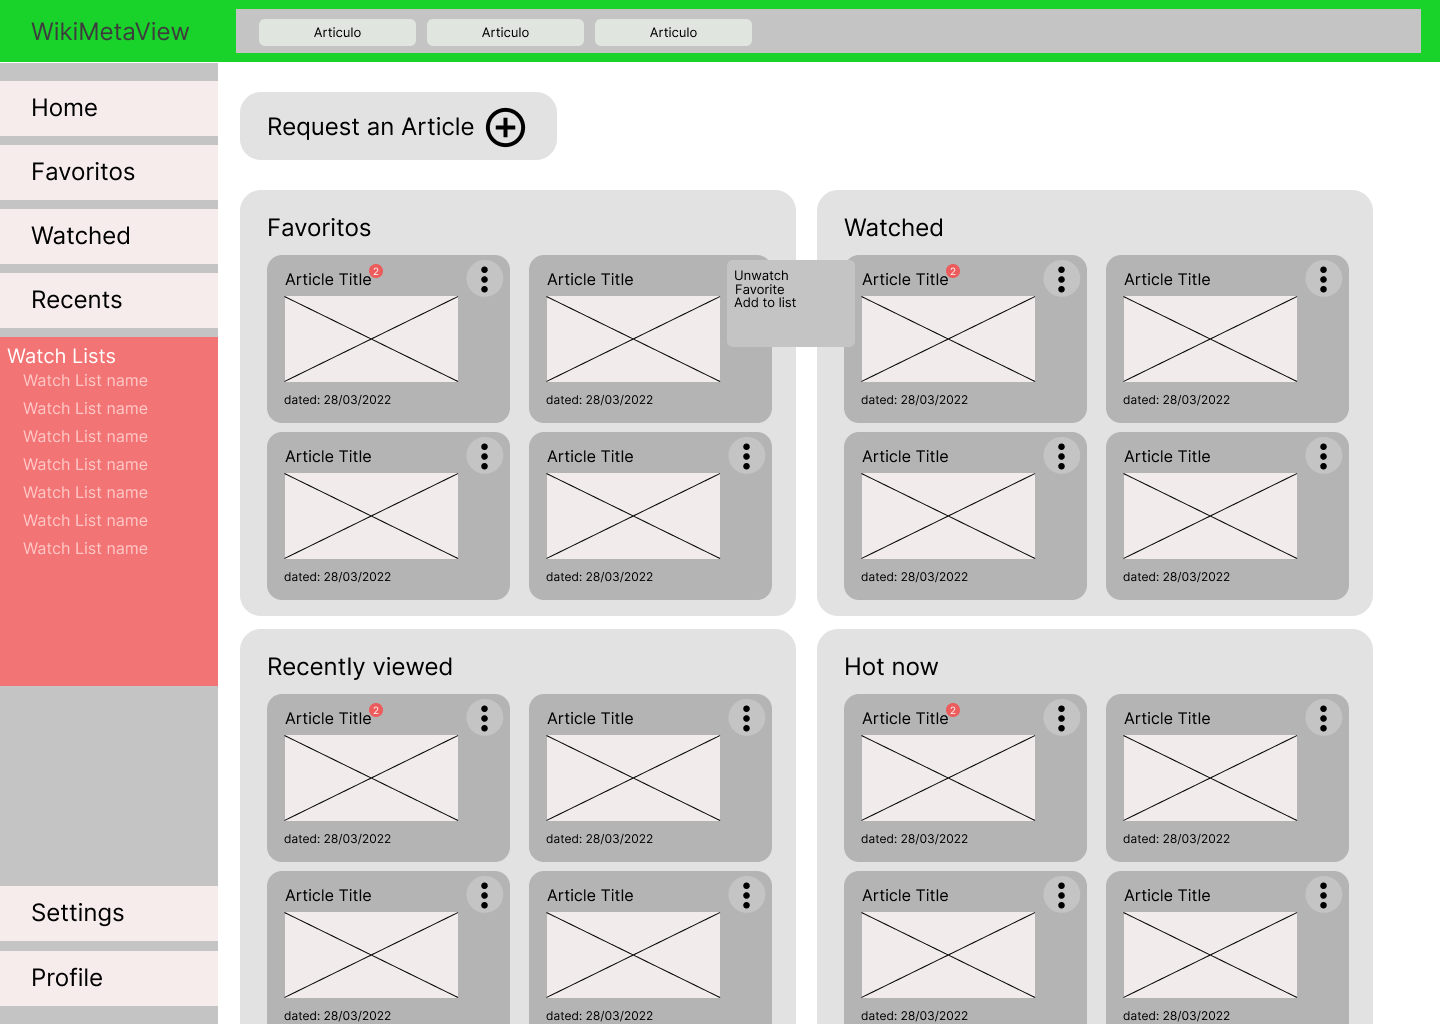
\includegraphics[width=1.0\textwidth]{prototipos/Index Auth.png}
    \caption{Prototipo de vista principal de un usuario autenticado}
    \label{PrototipoHomePage}
\end{figure}


Secciones del home
\begin{enumerate}
    \item Watched \\ Muestra una lista y un pequeño abstracto de los artículos que el usuario hace watching y tienen una visualización actualizada
    \item Queue \\ Muestra una lista de los artículos que el usuario solicito para hacer una visualización pero que el server no ha podido solicitar
    \item Controversial \\ Muestra una lista de aquellas visualizaciones que provocan discusión en la comunidad, caracterizado por muchos comentarios
\end{enumerate}

\subsection{Landing page \textbackslash}
TODO: poner imagen
Esta página se encarga de explicar las motivaciones de la App y dar una noción básica del funcionamiento para los watchers.
Tiene el objetivo de cap

\subsection{Página de configuración \textbackslash settings}
TODO: Terminar seccion de settings
Acá el usuario puede bla bla

\subsection{Página de artículo \textbackslash article}
\url{/article?title=<title>&url=<url>}
Muestra un artículo junto con su metadata y las visualizaciones creadas por los usuarios.

\begin{figure}[H]
    \centering
    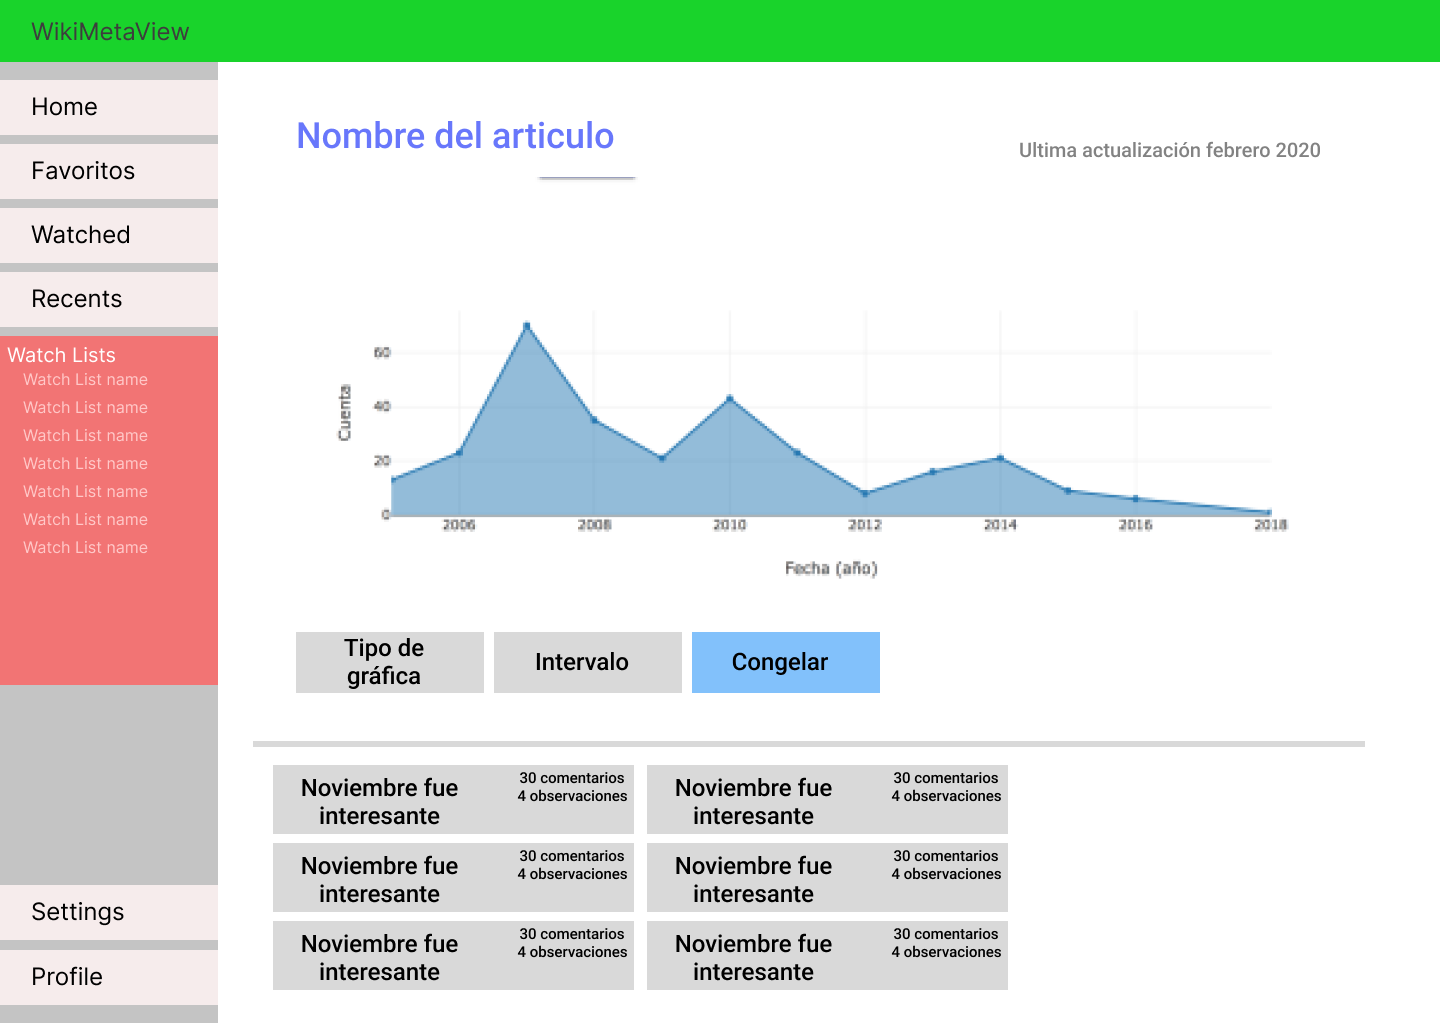
\includegraphics[width=1.0\textwidth]{prototipos/Article Page.png}
    \caption{Prototipo de página de artículos}
    \label{PrototipoSettingsPage}
\end{figure}

\subsection{Sobre nosotros \textbackslash about}
Breve resumen del proyecto, incluye el documento de tesis y documento de seminario así como datos de contacto y repositorios de github para futuros contribuyentes.

\section{Modales}
Las modales pueden sobreponerse a cualquier página en la aplicación y permiten al usuario efectuar una acción.

Estas modales serán controladas por parámetros de consulta agregados al URL de cada página web
CleanArquitecture
\subsection{Modal de autenticación}

Si este parámetro está en el URL. Presenta la modal de autenticación

\begin{figure}[H]
    \centering
    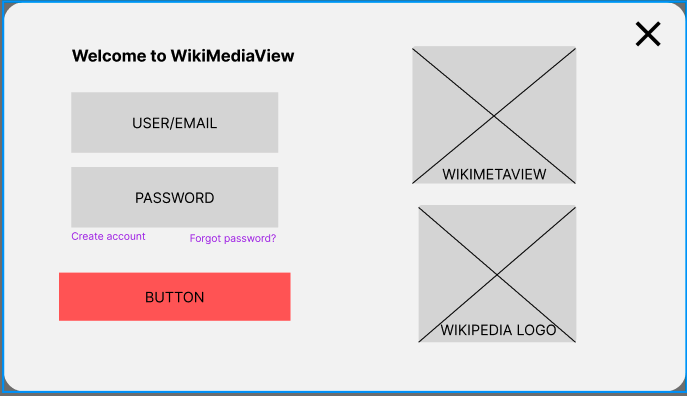
\includegraphics[width=1.0\textwidth]{prototipos/Modal-Auth.png}
    \caption{Modal de autenticación}
    \label{ModalAuth}
\end{figure}
?auth=true

\section{Planificación de las actividades}

TODO: UNA TABLA DE DOS COLUMNAS

ACTIVIDAD, TIEMPO ESTIMADO.

\begin{lstlisting}
    Preparar el entorno de desarrollo 1/2 semana
    Estudiar API Wikimetrics 2.0 (Back-end) 1/2 semana
    Estudiar API MediaWiki 1/2 semana
    Integracion del API Wikimetrics 2.0 (Back-end) 1/2 semana
    Integracion del API MediaWiki 1/2 semana
\end{lstlisting}